\documentclass[a4paper,10pt]{article}

\usepackage[latin1]{inputenc}
\usepackage{amsfonts}
\usepackage{amsmath}
\usepackage{amssymb}
\usepackage{amsthm}
\usepackage[T1]{fontenc}
\usepackage[dvips]{graphicx}

\author{Kefei Lu}
\title{The Blahut Algorithm For Estimating Channel Capacity}
\date{2008-05-05}

\begin{document}

\maketitle

%\begin{abstract}
%The report mainly illustrate how the Blahut algorithm for estimating channel capacity is implemented. 
%\end{abstract}

\section{Introduction}
% Here we illustrate the algorithm. Give flow charts. etc.
Blahut Algorithm is an iterative way to estimate the channel capacity and rate-distortion functions in information theory. 

In this project, the Blahut algorithm for estimating capacity-expense function is implemented using C programming language. The algorithm is implemented in an object-oriented fashion and is easy to use. The vector and matrix manipulation is based on the GNU Scientific Library. The algorithm is provided as a programming library so that it can be easily integrated in any other applications. The source code can be found on http://code.google.com/p/blahut/.

Figure \ref{fig:unconstrained_cap},\ref{fig:constrained_cap} show the algorithm for estimating the unconstrained capacity and the constrained capacity. They were originally published in R.E.Blahut's paper \textit{Computation of Channel Capacity and Rate-Distortion Functions} in 1972. 

The rest of the report is organized as following. Section \ref{sec:case_study} gives three examples to validate the implementation of the algorithm. Section \ref{Sec:Library_Use} illustrate how to install and use the library. Section \ref{sec:source} gives part of the library source codes that implement the Blahut algorithm.

\begin{figure}
 \centering
 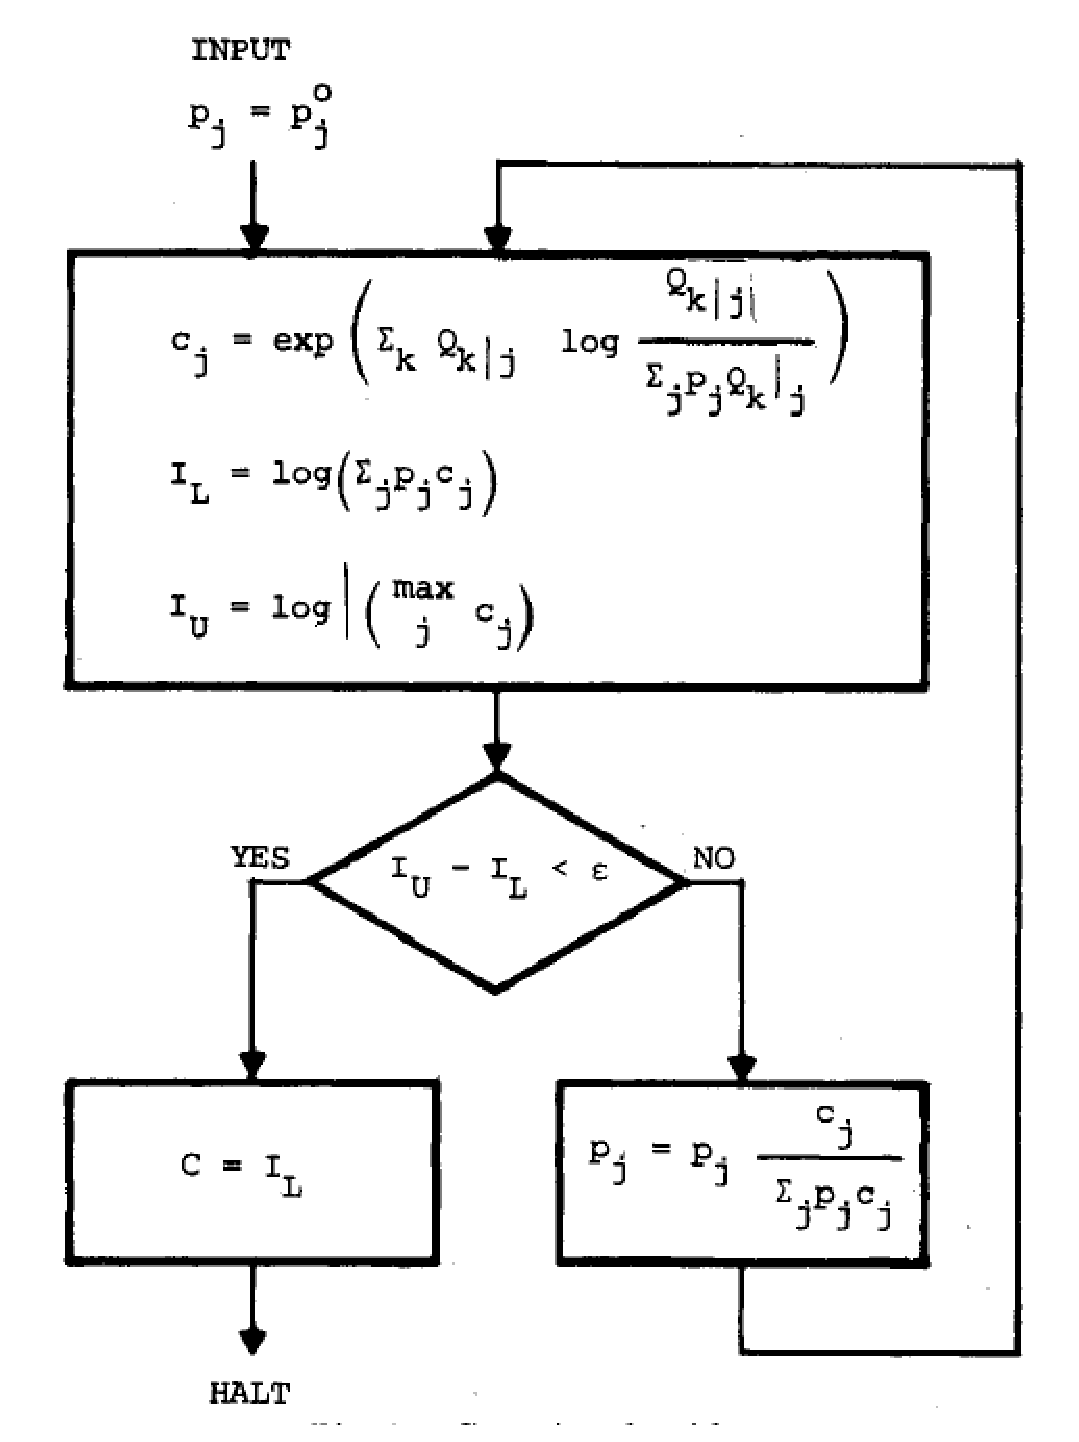
\includegraphics[width=0.5\textwidth]{pic/unconstrained_cap.eps}
 % unconstrained_cap.eps: 1179666x1179666 pixel, 300dpi, 9987.84x9987.84 cm, bb=14 14 516 690
 \caption{Flow chart illustration for computing unconstrained channel capacity}
 \label{fig:unconstrained_cap}
\end{figure}
\begin{figure}
 \centering
 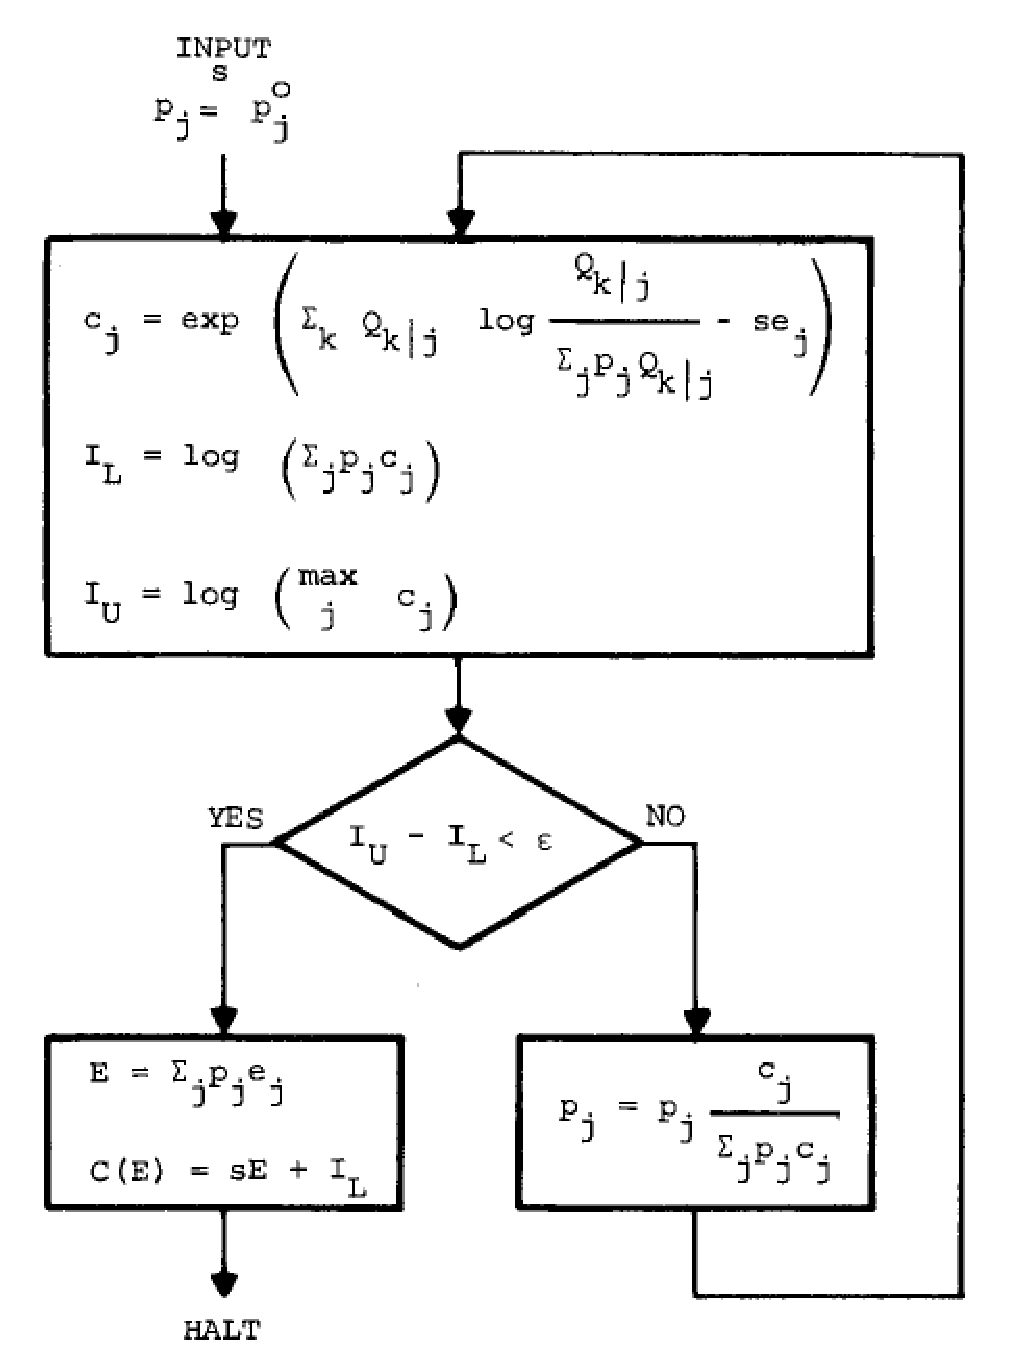
\includegraphics[width=0.5\textwidth]{pic/constrained_cap.eps}
 % unconstrained_cap.eps: 1179666x1179666 pixel, 300dpi, 9987.84x9987.84 cm, bb=14 14 516 690
 \caption{Flow chart illustration for computing constrained channel capacity}
 \label{fig:constrained_cap}
\end{figure}

\section{Case Study}
\label{sec:case_study}
% Describe the problem. Analize theoretically first, then show algorithm results.
\subsection{Binary Symmetric Channel}
The forward transition matrix of a binary symmetric channel can be expressed as:
\[\mathbf{Q} = \left[
\begin{array}{ccc}
1-p & p \\
p & 1-p \\
\end{array}
\right],\]
where $p$ is the cross over probability.

The unconstrained capacity is defined as:
\begin{equation}
 C = \max_{\mathbf{p}}{I(X,Y)}
\end{equation}
and is maximized to:
\begin{equation}
 C = 1 - \mathcal{H}(p), 
\end{equation}
when the input distribution is uniform distribution: $p^* = [0.5,0.5]^T$. 

For a special case when the cross-over probability $p=0$, i.e., all bits are transmitted reliably, $C = 1-\mathcal{H}(0) = 1\ bits/c.c$.

Given an expense schedule $\mathbf{e}$, and a constraint on the average expense of input $\sum_{x}{p(x)e(x)}\leq E$, the constrained capacity can be defined as:
\begin{equation}
 C(E) = \max_{\mathbf{p}\in P_E} {I(X;Y)} = \max_{\mathbf{p}\in P_E} {I(\mathbf{p};\mathbf{Q})},
\end{equation}
where $P_E$ is the constrained set and is defined as:
\begin{equation}
 P_E = \left\lbrace \mathbf{p}: p(x)\geq 0, \sum_{x}{p(x)}=1, \overline{E}=\sum_{x}{p(x)e(x)} \leq E \right\rbrace 
\end{equation}
If the expense schedule is set to $e=[0\ 1]^T$ for the BSC, we have $E_{min}=0$ when $\mathbf{p}=[1,\ 0]^T$, i.e., only $X=0$ is transmitted to avoid any expense on transmission. Thus we expect that the corresponding channel capacity $C_{min}=0$ because no information is conveyed in the transmission. Likewise, $C_{max}=1-\mathcal{H}(p)\ bits/channel\ use$ is achieved when $p^*_{\ E_{max}}=p^*=[0.5\ 0.5]^T$. And $E_{max}=0.5$.

For any $E\in[E_{min},\ E_{max}]$, since $p^*=[1-\alpha,\ \alpha]^T$, we have $\alpha=E$, therefore $p^*=[1-E,\ E]^T$. And the corresponding channel capacity can be expressed as
\begin{equation}
 C=I(\mathbf{p};\mathbf{Q})=\sum_{x}{p_x {\sum_{y} {p_{y|x}\log{\frac{p_{y|x}}{p_y}}}}}\ .
\end{equation}

Figure \ref{fig:bsc_cap} shows the result obtained by running the Blahut algorithm in the binary symmetric channel case, and $e=[0,\ 1]^T$. Different cross-over probabilities are tried and plotted on the same figure.
\begin{figure}
 \centering
 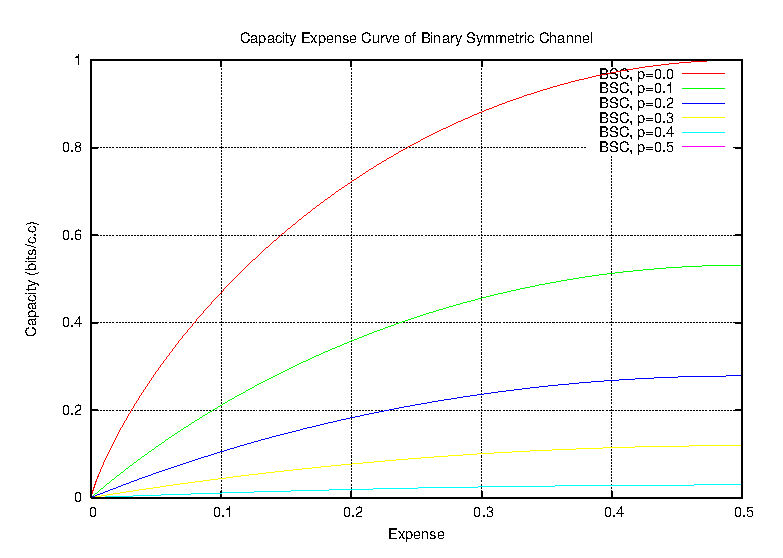
\includegraphics{pic/bsc_cap.eps}
 % bsc_cap.eps: 1179666x1179666 pixel, 300dpi, 9987.84x9987.84 cm, bb=50 50 410 302
 \caption{Capacity Expense Curve of Binrary Symmetric Channel for different cross-over probabilities. $e=[0\ 1]^T$}
 \label{fig:bsc_cap}
\end{figure}

\subsection{Example 1}
The forward transition matrix looks like the following:
\[
 \mathbf{Q} = \left[ 
\begin{array}{cccc}
1 & 0 & 0 & 0 \\ 
0 & q & 1-q & 0 \\ 
0 & 0 & 0 & 1
\end{array}\right] 
\]

As can be observed, $H(X|Y)=0$, i.e., when output is observed, the input can be uniquely determined. This is because that channel can be viewed as three parallel reliable subchannels. As can be expected, changing on parameter $q$ has no effect on the overall channel capacity.

The unconstrained capacity can be calculated as the following:
\begin{equation}
 C=\max_{\mathbf{p}} {I(X;Y)}=\max_{\mathbf{p}} {H(X)-H(X|Y)},
\label{eq:ex1_C}
\end{equation}
since $H(X|Y)=0$, eq. \ref{eq:ex1_C} can be further written as:
\begin{equation}
 C=\max_{\mathbf{p}}{H(X)},
\end{equation}
$H(X)$ is maximized when $\mathbf{p}=[1/3\ 1/3\ 1/3]^T$. And $C=\log_2{3}\approx1.59\ bits/channel\ use$.

When $e=[0,1,0]^T$ is assigned as expense schedule, $E_{min}$ is achived when $p=[\alpha/2\ 0\ \alpha/2]^T$, because of channel symetry. $C_{min}=log_2{3}\ bits/channel\ use$ as the channel reduces to BSC in this case.

Naturally, $C_{max}=C_{unconstrained}$ is achieved as $\mathbf{p}=[1/3\ 1/3\ 1/3]^T$. Therefore $E_{max}=1/3$ in this case.

Figure \ref{fig:example1_cap} shows the Blahut algorithm estimation on this channel for expense schedule $e=[0,1,0]^T$.
\begin{figure}
 \centering
 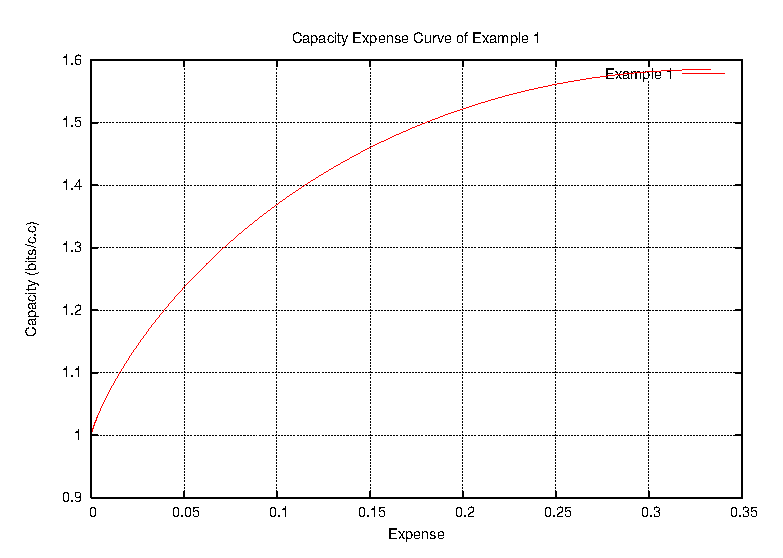
\includegraphics{pic/example1_cap.eps}
 % example1_cap.eps: 1179666x1179666 pixel, 300dpi, 9987.84x9987.84 cm, bb=50 50 410 302
 \caption{Capacity Expense Curve of Channel Described in Example 1. $e=[0,1,0]^T$.}
 \label{fig:example1_cap}
\end{figure}
As shown in the figure, the estimation agrees with theoretical analyse perfectly.

\subsection{Example 2}
The forward transition matrix looks like:
\begin{displaymath}
% use packages: array
\mathbf{Q}=\left[ 
\begin{array}[c]{ccc}
1-p & p & 0 \\ 
0 & 1 & 0 \\ 
0 & p & 1-p
\end{array}\right], 
\end{displaymath}
with expense schedule $e=[1,0,1]^T$.

It's easy to show from Kuhn-Tuckor condition that the unconstrained capacity can be achieved when $p^*=[\frac{1-\alpha}{2}\ \alpha \frac{1-\alpha}{2}]^T$. The unconstrained capacity is
\begin{equation}
 C=log{\frac{1/p}{1+\alpha^*\left(\frac{1-p}{p}\right)}}
\end{equation}

For example, $p=1/3$, we solve for
\begin{equation}
 \frac{1-\alpha}{1+2\alpha}=2\left(\frac{1}{3}\right)^{3/2}
\end{equation}
in which case
\[\alpha^*=\frac{3\sqrt{3}-2}{3\sqrt{3}+4}\approx0.348\],
and 
\[C=log{\frac{3}{1+2\alpha^*}}\approx0.824\ bits/channel\ use\].

Now let's consider capacity expense function C(E). Clearly we have $E_{min}=0$ which is achieved when $p_{E_{min}}^*=[0,1,0]^T$. The corresponding capacity is $C(E_{min})=0$.

For $E\geq0$, $p_E^*=[\frac{1-\alpha_E^*}{2},\alpha_E^*,\frac{1-\alpha_E^*}{2}]^T$, due to channel symmetry. Since $1-\alpha_E^*=E$, we have
\begin{equation}
 p_E^*=[E/2,1-E,E/2]^T
\end{equation}
Finally we have
\begin{equation}
 C(E)=I(p_E^*;Q)=H(Y)-H(Y|X)=E(1-p)+\mathcal{H}(E(1-p))-E\mathcal{H}(p)
\end{equation}
For different value of $p$, we have different $C(E_{max})$ and the corresponding $E_{max}$. For the example that $p=1/3$, we have $C(E_{max})\approx0.824$, when $E_{max}=1-\alpha^*\approx0.652$. 

The case when $p=1/3$ is estimated using Blahut algorithm and is shown in figure \ref{fig:example2_p0.3}. Also, cases with different $p$ values are plotted together in figure \ref{fig:example2_cap}.

\begin{figure}
 \centering
 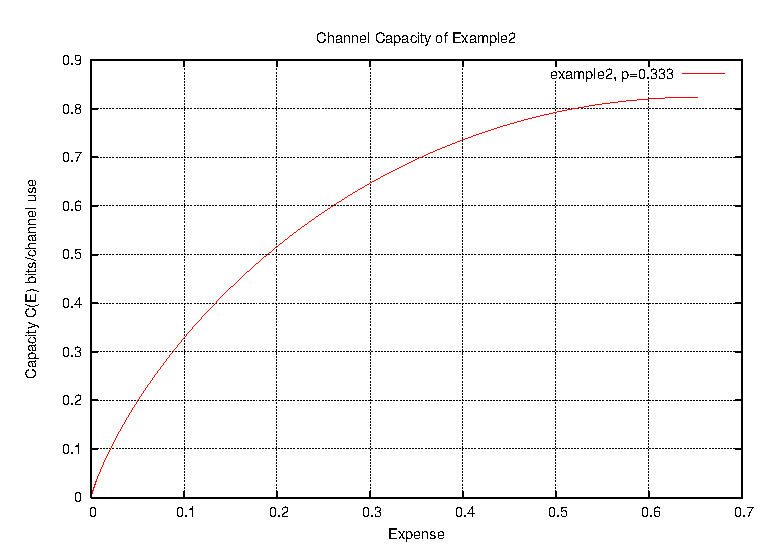
\includegraphics{pic/example2_cap_p0.3.eps}
 % example2_cap_p0.3.eps: 360x252 pixel, 72dpi, 12.70x8.89 cm, bb=0 0 360 252
 \caption{Capacity Expense Curve of Example 2 with p=1/3}
 \label{fig:example2_p0.3}
\end{figure}

\begin{figure}
 \centering
 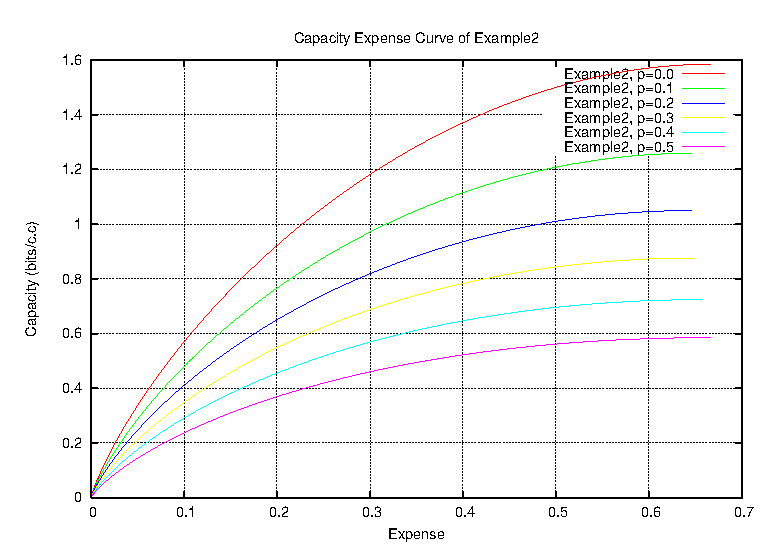
\includegraphics[bb=50 50 410 302]{pic/example2_cap.eps}
 % example2_cap.eps: 1179666x1179666 pixel, 300dpi, 9987.84x9987.84 cm, bb=50 50 410 302
 \caption{Capacity Expense Curve of Example 3 with different values of p}
 \label{fig:example2_cap}
\end{figure}

\section{Library Usage}
\label{Sec:Library_Use}
% Manual for the library.
\subsection{Installation}
To use the library, one must have GNU Scientific Library (GSL) installed. GSL is used in this library for mathematical and matrix manipulations. In fact, this library is intend to be an extension of GSL. 

Two optional software are GNU Plot and GNU Octave, which are used to plot the curves.

To build the library, copy it to the desired location, and type \verb|make| to build the shared library file ``libblahut.so''. To link with this library, one must:
\begin{enumerate}
 \item Include \verb|blahut.h| in the source files
 \item Include /path/to/lib (path where ``libblahut.so'' locates) to the \verb|LD_LIBRARY_PATH| environment
 \item At the link stage, append linking options 
\begin{verbatim}
-L/path/to/lib -lm -lblahut `gsl-config --libs`
\end{verbatim}
 to the linker command
\end{enumerate}
\verb|make clan| will clean all the built objects and executables.

An alternative way to use the library is even more straightforward: just compile the blahut.c to blahut.o, and then link the object file together with other objecte files. Note that when linking all the object files, append the option \verb|`gsl-config --libs`| to the linker, as GSL is used in the algorithm.

\subsection{Objects and Meathods}
The library was written in C programming language, in an object-oriented fashion. The main manipulating object type is structure \verb|blahut_cap|, which contains all the setting parameters and resulting data.

The following functions are provided to manipulating an object of type \verb|blahut_cap|.
\begin{verbatim}
blahut_cap * 
blahut_cap_init( const gsl_matrix* Q, 
		   const gsl_vector* e );
\end{verbatim}
This function takes a forward transition matrix (of type \verb|gsl_matrix|) and an expense schedule (of type \verb|gsl_vector|) as arguments, and returns a pointer to an initialized (dynamically allocated) object of type \verb|blahut_cap|, which will be used for further specifying channel and algorithm parameters, storing estimated data.

\begin{verbatim}
void 
blahut_cap_free( blahut_cap* cap);
\end{verbatim}
Since \verb|blahut_cap| is dynamically allocated, never forget to free the memory after using it. \verb|blahut_cap_free()| takes a pointer to a capacity object and frees the corresponding object and all the relavant memory.
Note: do not free this pointer by using \verb|free()| from standard C, as some pointers in that object also pointing to dynamically allocated memory blocks.

\begin{verbatim}
blahut_cap * 
blahut_cap_setSRange(blahut_cap * cap, double s_L, double s_U, double step);
\end{verbatim}
After an \verb|blahut_cap| object has been initialized, this function is used to set the $s$ ranges (refer to figure \ref{fig:constrained_cap}) to obtain a series of points on the C(E) curve. Different $s$ value corresponds to expenses, $s=0$ corresponds to unconstrained (or $E_{max}$) case.

\begin{verbatim}
blahut_cap *
blahut_cap_calc( blahut_cap * cap );
\end{verbatim}
When given a specific $s$, this function iterates and estimates a corresponding capacity.

\begin{verbatim}
blahut_ce_curve 
blahut_cap_iterate_over_s( blahut_cap * cap, const char* filename);
\end{verbatim}
After setting the $s$ range, this function starts iterating over all $s$ values by calling \verb|blahut_cap_calc()| function repeatedly.

\subsection{Utilities}
\subsubsection{Demos}
The three examples illustrated in section \ref{sec:case_study} are provided as demos in subdirectory examples/. To build the examples, type command \verb|make examples|, to demonstrating examples, type commands: \verb|./bscDemo|, \verb|./example1Demo|, \verb|example2Demo| respectively. Note that to use the demos, make sure GNU Plot and GNU Octave are installed correctly.

\subsubsection{Calculating Binary Entropy Function}
A small utility is provided to compute the binary entropy function $\mathcal{H}(.)$. To invoke the utility, \verb|cd| to subdirectory bin/, and execute command \verb|./binary_entropy p|, where $p$ is a real number between 0 and 1.

\section{Library Source Codes}
\label{sec:source}
\subsection{blahut.h}
\begin{verbatim}
#include <stdio.h>
#include <stdlib.h>
#include <limits.h>
#include <math.h>
#include <string.h>

#include <gsl/gsl_vector.h>
#include <gsl/gsl_matrix.h>

#ifndef __BLAHUT_H__
#define __BLAHUT_H__

/*
 * This type is used to determine the unit used to measure information.
 */
typedef enum {
    BITS, 
    NATS
} blahut_unit;

/* This structure stores the estimated capacity-exapense curve
 * and the optimizing input probability distribution.
 * The length of the three vectors are the same. */
struct blahut_ce_curve_str {
    unsigned int len;
    gsl_matrix * p;
    gsl_vector * E;
    gsl_vector * C;
};
typedef struct blahut_ce_curve_str blahut_ce_curve;

struct blahut_constrained_capacity {
    /* Unit used to express the channel capacity */
    blahut_unit	unit;
    /* These two members must be specified */
    gsl_matrix *	Q;	/* the foward transition matrix */
    gsl_vector *	e;	/* the expense vector */

    gsl_vector *	p;	/* the source probability distribution */
    gsl_matrix *	P;	/* the backward transition matrix */
    gsl_vector *	c;	/* the capacity vector c_j */

    /* A M x (2+numIn) matrix storing the Expense and corresponding Capacity, 
     *   and the maximizing p vector. M = floor((s_U - s_L)/s_d). 
     * Only used when iterating over s, DO NOT use this varaible otherwise. */
    /*
    gsl_matrix *	ce_curve;	
    */
    blahut_ce_curve 	ce_curve;

    int		numIn;	/* This is the # rows in Q matrix
				   and the # col. in P matrix */
    int 	numOut;	/* This is the # col. in Q matrix 
				   and the # rows in P matrix */

    double 	I_L;	/* the lower bound of I */
    double 	I_U;	/* the upper bound of I */
    double 	E;	/* the Expense */
    double 	C;	/* the Capacity */

    double 	s;	/* the parameter s */
    /* These three are only used when calculate the C(E) curve 
     * (iterates on s) */
    double	s_L;	/* the lowest value of s */
    double 	s_U;	/* the highest value of s */
    double 	s_d;	/* the iteration step on s */


    double 	epsilon;/* the error toleration */

    unsigned int	it;	/* the interation index */
    unsigned int	maxNumIt; /* the max # of iterations allowed.
				     The default value set in 
				     blahut_cap_init() is 
				     the limit of unsigned int: UINT_MAX */
    int		exceedsMaxNumIt;  /* this flag is set to true if after maxNumIt 
				     iterations, the terminating creteria still 
				     haven't been met. */
};
typedef struct blahut_constrained_capacity blahut_cap; /* a shorthand */

blahut_cap * 
blahut_cap_init( const gsl_matrix* Q, 
		   const gsl_vector* e );

void 
blahut_cap_free( blahut_cap* cap);

/*
blahut_cap * 
blahut_cap_set_p( blahut_cap * cap,
		    const gsl_vector* p );
*/

blahut_cap *
blahut_cap_calc( blahut_cap * cap );

blahut_cap * 
blahut_cap_set_p_uniform( blahut_cap * cap );

blahut_ce_curve 
blahut_cap_iterate_over_s( blahut_cap * cap, const char* filename);

blahut_cap * 
blahut_cap_setSRange(blahut_cap * cap, double s_L, double s_U, double step);
#endif /*  __BLAHUT_H__ */

\end{verbatim}

\subsection{blahut.c}
\begin{verbatim}
#include <assert.h>
#include "blahut.h"
 
/* print useful information about what is going on */
#define DEBUG

/* print result in calculation for algorithm correctness check*/
/* #define DEBUG_Calc */

/* print warning message */
#define DEBUG_PRINT_WARNING 

/* Maximum amount of iteration allowed in calculating a point on C(E) curve */
#define DEFAULT_MAX_IT UINT_MAX

/* The range within wich 2 double values are judged as the same */
#define DOUBLE_COMP_LIMIT 1e8

/* 
 * Many systems already have my_log2 function. If not, remove the 
 * ifdef, endif preprocessor to enable this function.
 */
inline static double my_log2(const double value)
{
    return log10(value)/log10(2);
}

/*
 * Natural Logarithm.
 */
inline static double my_loge(const double value)
{
    return log(value);
}

static int 
vector_isnonneg(const gsl_vector* vec)
{
    unsigned int i;
    for (i=0;i<vec->size;i++) {
	if (gsl_vector_get(vec,i) < 0) {
	    return 0;
	}
    }
    return 1;
}

static int 
matrix_isnonneg(const gsl_matrix* mat)
{
    unsigned int j,k;
    for (j=0;j<mat->size1;j++) {
	for (k=0;k<mat->size2;k++) {
	    //printf("%g\n",gsl_matrix_get(mat,j,k));
	    if (gsl_matrix_get(mat,j,k) < 0.0) {
		return 0;
	    }
	}
    }
    return 1;
}

blahut_cap * 
blahut_cap_init( const gsl_matrix* Q, 
		   const gsl_vector* e )
{
    unsigned int i=0, k=0;
    blahut_cap * cap = (blahut_cap*) malloc (sizeof(blahut_cap));
    if (!cap) {
	fprintf(stderr, "(E) Not enough memory when allocating a blahut_cap.\n");
	exit(1);
    }
    memset(cap, 0, sizeof(blahut_cap));

    /* Check validity of Q and e */
    if (Q == NULL || e == NULL) {
	fprintf(stderr, "(E) Q or e is NULL pointer.\n");
	exit(1);
    }
    if (Q->size1 != e->size) {
	fprintf(stderr, "(E) Q's # rows is not equal to e's size.\n");
	exit(1);
    } else if (Q->size2 <= 0) {
	fprintf(stderr, "(E) Q's # columns should not be negative.\n");
	exit(1);
    } else if (!vector_isnonneg(e) || !matrix_isnonneg(Q)) {
	fprintf(stderr, "(E) Q or e contains negative elements.\n");
	exit(1);
    }

    /* Check the validity of Q and e */
    double sum_Q=0;

    /* each row of Q should sum to 1 */
    for (i=0;i<Q->size1;i++) {
	sum_Q=0;
	for (k=0;k<Q->size2;k++) {
	    sum_Q += gsl_matrix_get(Q, i, k);
	}
	if (fabs(sum_Q - 1.0) > DOUBLE_COMP_LIMIT) {
	    fprintf(stderr, "(E) Sum over row %d of Q seems not to be 1.\n", k);
	    exit(2);
	}
    }

    cap->Q = (gsl_matrix*)Q;
    cap->e = (gsl_vector*)e;
    
    /* Process Q and e */
    cap->numIn = Q->size1;
    cap->numOut = Q->size2;

    /* Initialize p, P, c */
    cap->p = gsl_vector_alloc(cap->numIn);
    gsl_vector_set_all(cap->p, 1.0/cap->numIn); /* init. the input distribution
					      as uniform */
    cap->P = gsl_matrix_calloc(cap->numOut, cap->numIn); /* numOut x numIn */
    cap->c = gsl_vector_calloc(cap->numIn); /* numIn x 1 */

    /* The default values */
    cap->unit = BITS;
    cap->s_L = 0.0;
    cap->s_U = 1e4;
    cap->s_d = 0.001;

    cap->epsilon = 1e-5;
    cap->maxNumIt = DEFAULT_MAX_IT;

    return cap;
}

void 
blahut_cap_free( blahut_cap* cap)
{
    gsl_matrix_free(cap->P);
    gsl_vector_free(cap->p);
    gsl_vector_free(cap->c);
    if (cap->ce_curve.p) {
	gsl_matrix_free(cap->ce_curve.p);
    }
    if (cap->ce_curve.E) {
	gsl_vector_free(cap->ce_curve.E);
    }
    if (cap->ce_curve.C) {
	gsl_vector_free(cap->ce_curve.C);
    }

    free(cap);
}

/* Calculate:
 * sum_j {p_j * Q_{k|j}} */
inline static double
sum_p_Q (const blahut_cap * cap, int k)
{
    register int j = 0;
    register double sum = 0;
    for (j=0; j<cap->numIn; j++) {
	sum += gsl_vector_get(cap->p, j) * gsl_matrix_get(cap->Q, j, k);
    }
#ifdef DEBUG_Calc
    fprintf(stdout, "(I) q_Y[%d] = %g\n", k, sum);
#endif
    return sum;
}

/* Calculate the sum of the first term of exp(...) in c_j
 * expression */
inline static double 
sum_Q_log (const blahut_cap * cap, int j)
{
    register int k = 0;
    register double Q_kj;
    register double sum = 0;

    for (k=0; k<cap->numOut; k++) {
	Q_kj = gsl_matrix_get(cap->Q, j, k);
	/* use the convention that 0log0 = 0 */
	sum += (Q_kj == 0 ? 0 : Q_kj * my_loge (Q_kj/sum_p_Q(cap,k)));
    }

#ifdef DEBUG_Calc
    fprintf(stdout, "sum_k Q_k|%d * log(Q_k|%d/q_Y[k]) = %g\n",
	    j,j,sum);
#endif
    return sum;
}

/* Calculate c_j over all j */
static blahut_cap * calc_c_j ( blahut_cap * cap )
{
    int j;
    for (j=0; j<cap->numIn; j++) {
	gsl_vector_set(cap->c, j, 
		exp(sum_Q_log(cap, j)
		    - cap->s * gsl_vector_get(cap->e,j)));
#ifdef DEBUG_Calc
	fprintf(stdout, "(I) c[%d] = %g\n", j, gsl_vector_get(cap->c,j));
#endif
    }
    return cap;
}

inline static double calc_I_L (blahut_cap * cap)
{
    int j;
    double sum=0;
    for (j=0; j<cap->numIn; j++) {
	sum += gsl_vector_get(cap->p,j) * gsl_vector_get(cap->c,j);
    }
    cap->I_L = my_loge(sum);
    return cap->I_L;
}

inline static double calc_I_U (blahut_cap * cap)
{
    cap->I_U = my_loge(gsl_vector_max ( cap->c ));
    return cap->I_U;
}

static blahut_cap * update_p (blahut_cap * cap)
{
    double sum=0;
    int j;
    for(j=0;j<cap->numIn;j++) {
	sum += gsl_vector_get(cap->p,j) * gsl_vector_get(cap->c,j);
    }

    for (j=0;j<cap->numIn; j++) {
	gsl_vector_set(cap->p,j, 
		gsl_vector_get(cap->p,j)
		* (gsl_vector_get(cap->c,j) / sum));
    }

    return cap;
}

static double calc_E(blahut_cap * cap)
{
    int j;
    double sum = 0;
    for(j=0;j<cap->numIn; j++) {
	sum += gsl_vector_get(cap->p,j) * gsl_vector_get(cap->e,j);
    }
    cap->E = sum;
    return sum;
}

static double calc_C(blahut_cap * cap)
{
    cap->C = cap->s * cap->E + cap->I_L;

    if (cap->unit == NATS) {
	return cap->C;
    } else if (cap->unit == BITS) {
	cap->C = my_log2(exp(cap->C));
	return cap->C;
    } else {
	fprintf(stderr, "(W) Wrong information unit specified:%d, "
		"using the default: %d\n", cap->unit, BITS);
	cap->unit = BITS;
	calc_C(cap);
    }
    return cap->C;
}
    
blahut_cap *
blahut_cap_calc( blahut_cap * cap )
{
    for(cap->it=0 ; cap->it < cap->maxNumIt ; cap->it++ ) {
	calc_c_j(cap);
	if (calc_I_U(cap) - calc_I_L(cap) < cap->epsilon) {
	    calc_E(cap);
	    calc_C(cap);
	    break;
	} else if ( isnan(cap->I_U) || isnan(cap->I_L) ) {
#ifdef DEBUG_PRINT_WARNING
	    fprintf(stdout, "(I) I_U or I_L is NaN, terminate loop.\n");
#endif
	    break;
	}
	update_p(cap);
    }

    /* to check if for() is terminated by a break or by
     * cap->it >= cap->maxNumIt */
    if (cap->it >= cap->maxNumIt) {
	/* for() is terminated by exceeding the max # iterations */
	calc_E(cap);
	calc_C(cap);
	cap->exceedsMaxNumIt = 1;
    }

    return cap;
}

inline blahut_cap * 
blahut_cap_set_p_uniform( blahut_cap * cap )
{
    gsl_vector_set_all(cap->p, 1.0/cap->p->size);
    return cap;
}

static blahut_ce_curve * 
ce_curve_init( blahut_cap * cap )
{
    cap->ce_curve.len = (unsigned int)floor((cap->s_U - cap->s_L)/cap->s_d);
    cap->ce_curve.p = gsl_matrix_calloc(cap->ce_curve.len, cap->numIn);
    cap->ce_curve.E = gsl_vector_calloc(cap->ce_curve.len);
    cap->ce_curve.C = gsl_vector_calloc(cap->ce_curve.len);

    return &(cap->ce_curve);
}

blahut_ce_curve  
blahut_cap_iterate_over_s( blahut_cap * cap, const char* filename)
{
    /* Initialize the field 'cap->ce_curve' for storing data */
    ce_curve_init(cap);

#ifdef DEBUG
    fprintf(stdout, "(I) Calculating C(E) curve ...\n");
#endif

    unsigned int NumS = cap->ce_curve.len; /* # samples on the curve */
    unsigned int i,j;
    double step = cap->s_d;
    /* Begin iterating over s */
    for (i=0,cap->s = cap->s_L; i<NumS; i++, cap->s+=step) {
	//printf("%d, %g\n",i,cap->s);
	blahut_cap_set_p_uniform(cap);
	blahut_cap_calc(cap);

	/* stop iterating */
	if (cap->C == 0 || cap->E == 0) {
#ifdef DEBUG_PRINT_WARNING
	    fprintf(stdout, "(W) C = 0 or E = 0 encountered, break the iteration.\n");
#endif
	    break;
	}

	/* Store the result */
	{
	    gsl_vector_view p_view = gsl_matrix_row(cap->ce_curve.p, i);
	    gsl_vector_memcpy(&p_view.vector, cap->p);

	    gsl_vector_set(cap->ce_curve.E, i, cap->E);
	    gsl_vector_set(cap->ce_curve.C, i, cap->C);
	}
    }
#ifdef DEBUG
    fprintf(stdout, "(I) Finished.\n");
#endif

    /* Write to file */
    if (filename != NULL) {
#ifdef DEBUG
	fprintf(stdout, "(I) Writing data to file ...\n");
#endif
	FILE * file = fopen(filename,"w");
	if (file == NULL) {
	    fprintf(stderr, "(E) Error opening file \"%s\" for writing.\n", 
		    filename);
	    exit(1);
	}
	for (i=0; i<NumS; i++) {
	    fprintf(file, "%g ", gsl_vector_get(cap->ce_curve.E, i));
	    fprintf(file, "%g ", gsl_vector_get(cap->ce_curve.C, i));
	    for (j = 0; j < cap->numIn; j++) {
		fprintf(file, "%g ", gsl_matrix_get(cap->ce_curve.p, i, j));
	    }
	    fprintf(file, "\n");
	}
	fclose(file);
#ifdef DEBUG
	fprintf(stdout, "(I) Finished.\n");
#endif
    }

    return cap->ce_curve;
}

blahut_cap * 
blahut_cap_setSRange(blahut_cap * cap, double s_L, double s_U, double step)
{
    if (s_U < s_L) {
	fprintf(stderr, "(E) blahut_cap_setSRange:" 
		"The upper limit %g is less than the lower limit %g.\n",
		s_U, s_L);
	exit(3);
    }
    cap->s_L = s_L;
    cap->s_U = s_U;
    cap->s_d = step;

    return cap;
}
\end{verbatim}
 
\end{document}
